\documentclass{standalone}

\begin{document}

\subsection[miRNA and RPPA data]{miRNA and RPPA dataset}\label{synapse:miRNA}

The same analysis pipeline presented in the paper about gene expression data from the Synapse dataset is applied in this Section also to the miRNA and RPPA datasets, with the results presented in Fig.~\ref{fig:other_results}.

\begin{figure}[htbp]
\centering
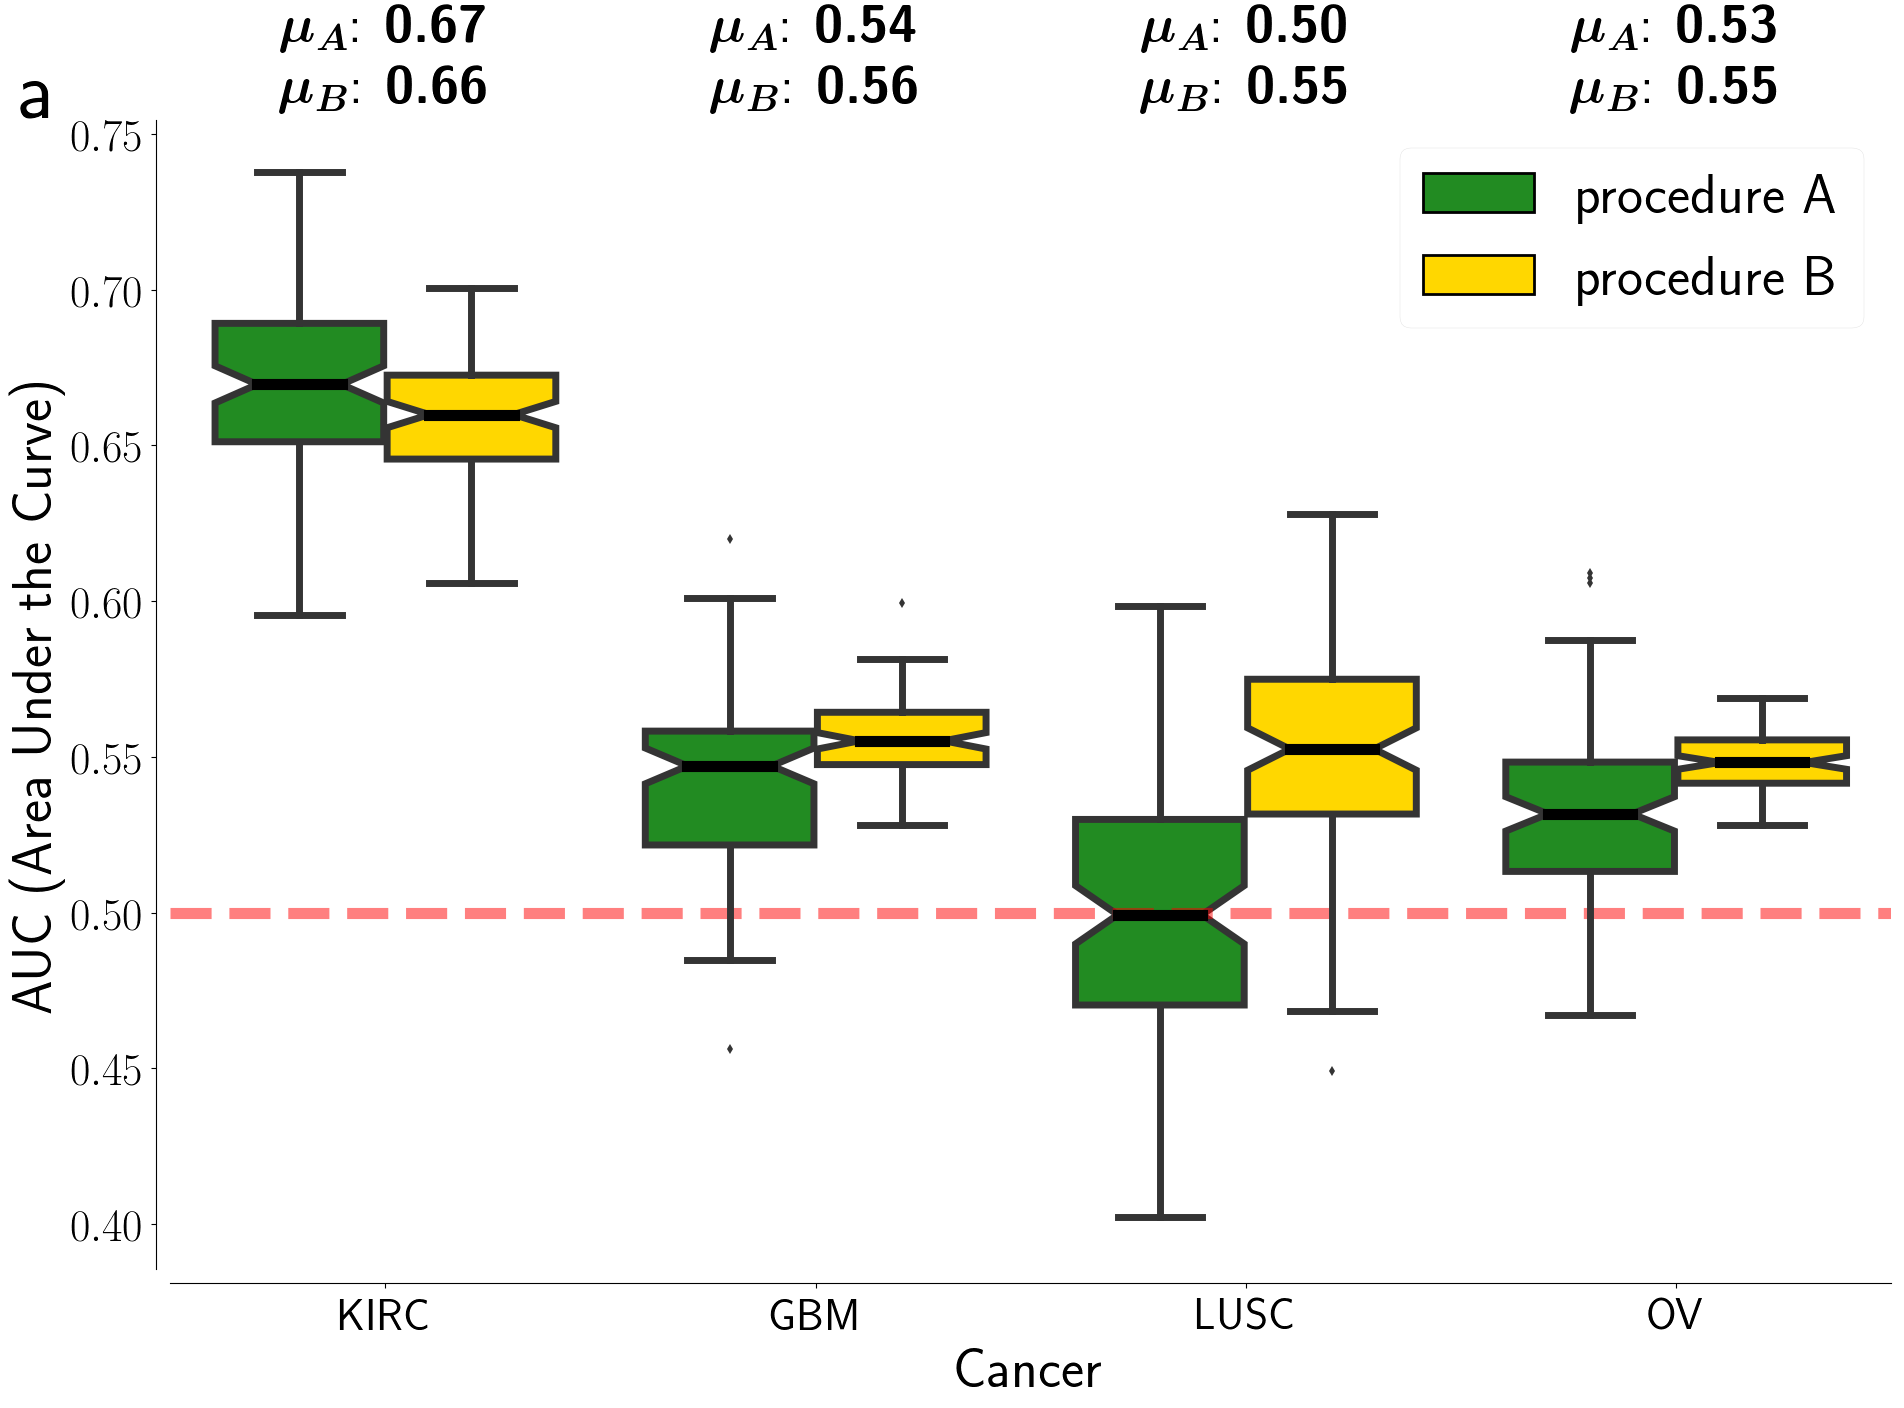
\includegraphics[width=0.4\textwidth]{miRNA_boxplot.png}
\qquad
\def\svgwidth{0.45\textwidth}
\input{./img/miRNA_tables.pdf_tex}
\newline
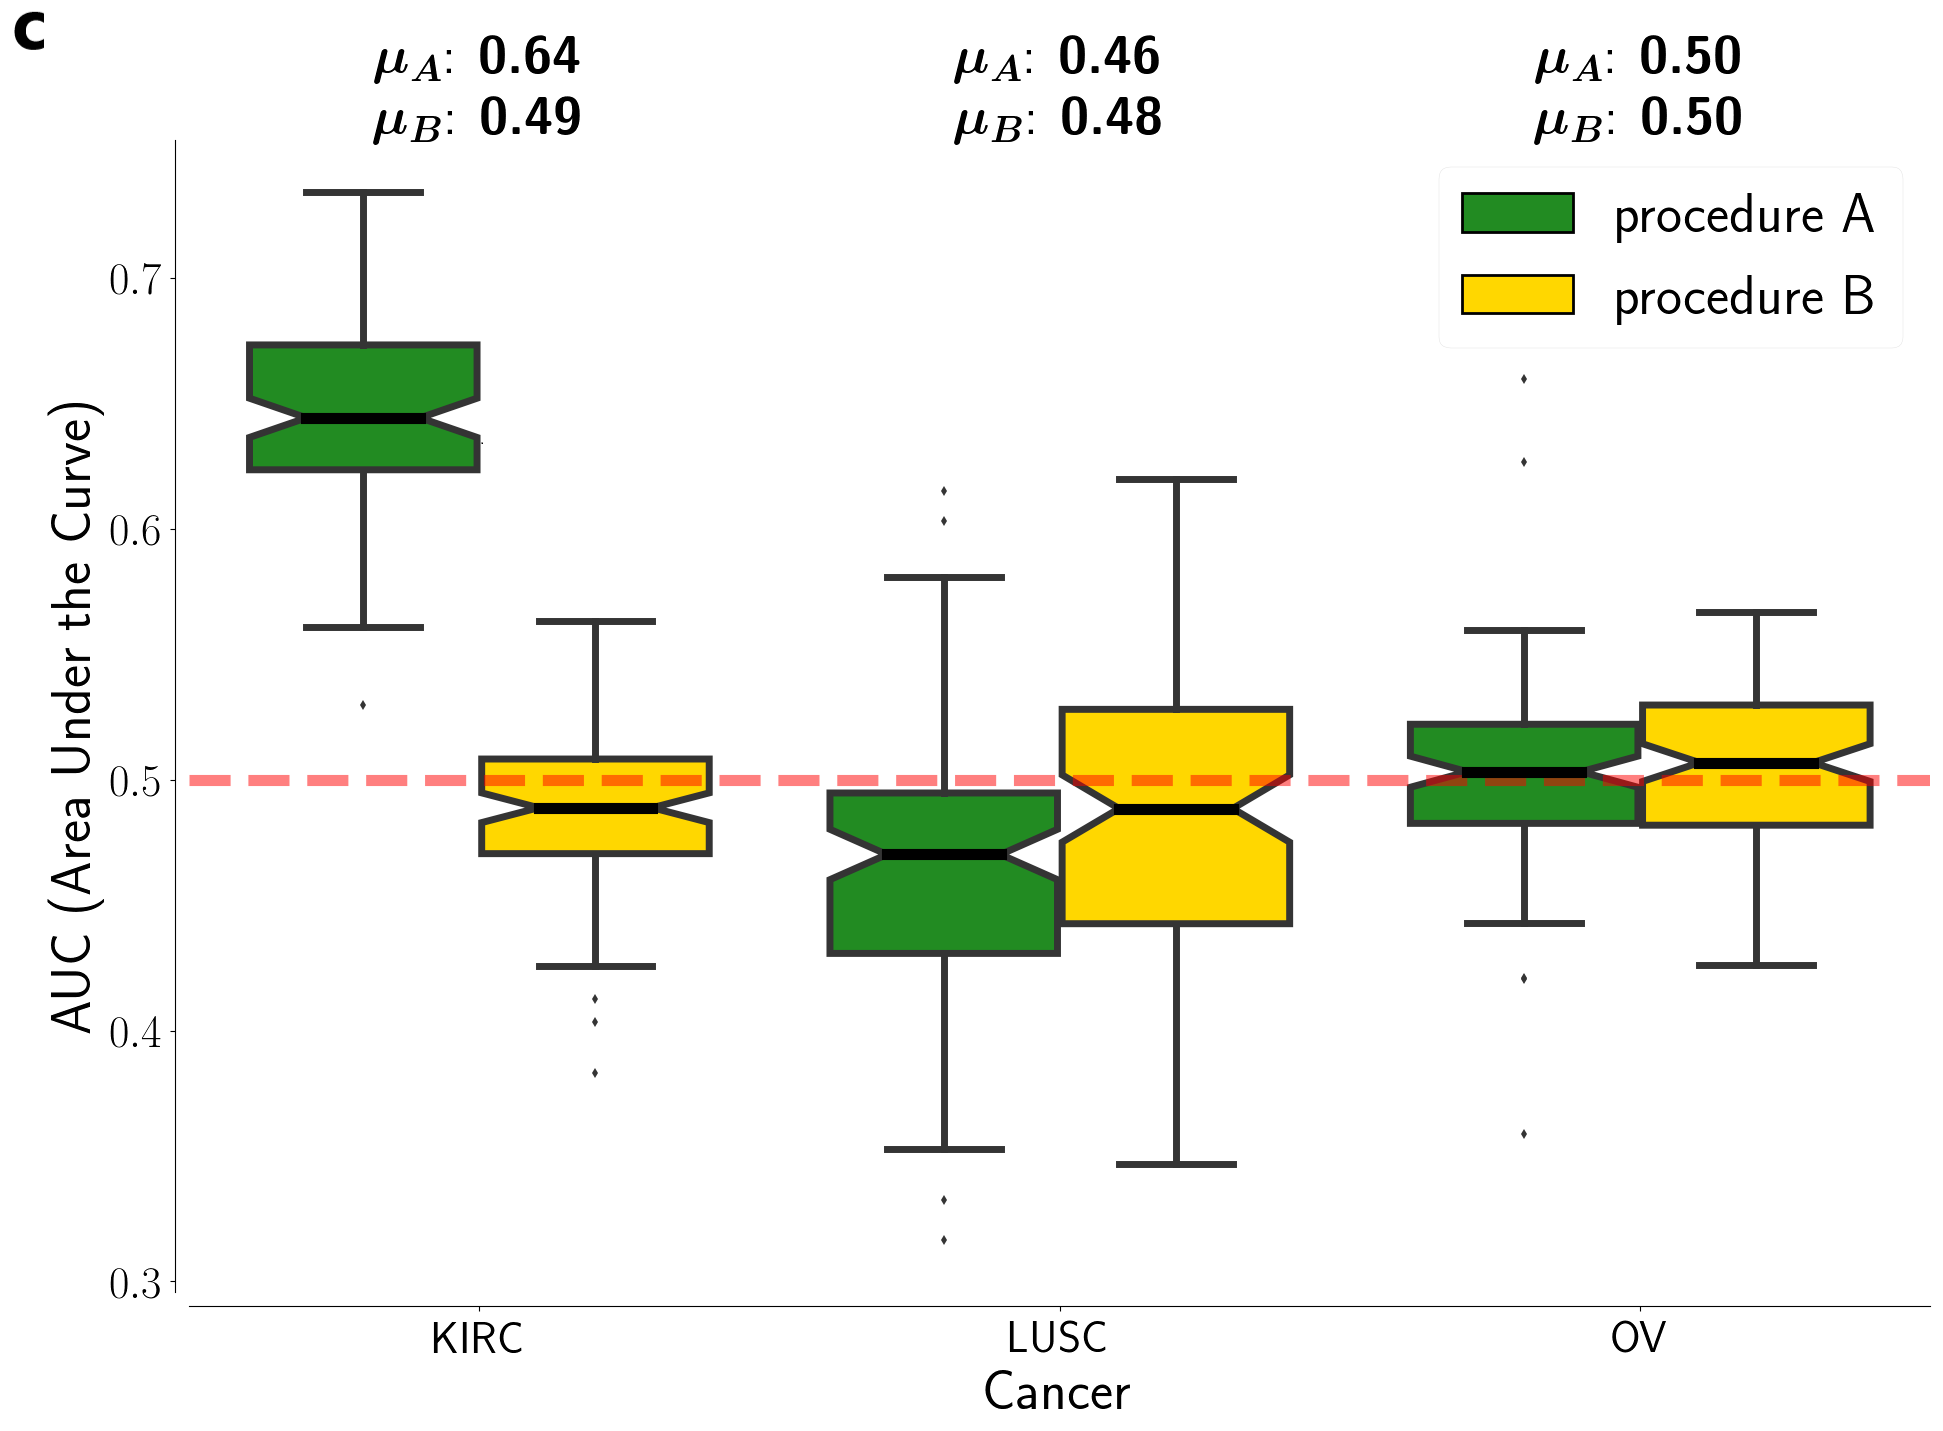
\includegraphics[width=0.4\textwidth]{RPPA_boxplot.png}
\qquad
\centering
\def\svgwidth{0.45\textwidth}
\input{./img/RPPA_tables.pdf_tex}
\caption{Results obtained by the \textsf{DNetPRO} algorithm pipeline on the four Synapse miRNA and RPPA tumors datasets.
\textbf{(a, c)} Distributions of AUC scores obtained over the four datasets.
Green box-plots: results using procedure $A$ of DnetPRO; yellow box-plots: results obtained using procedure $B$.
\textbf{(b, d)} Comparison of \textsf{DNetPRO} with the methods used in~\cite{Yuan2014}.
The reported values are the max AUC values obtained over the 10-Fold cross-validation procedure.
}
\label{fig:other_results}
\end{figure}

The results obtained on the miRNA dataset (Fig.~\ref{fig:other_results} (a, b)) are comparable to the reference, while for the RPPA dataset only the LUSC tumor shows AUC values comparable with the others.
Moving from the procedure $A$ to the procedure $B$, i.e. adding a second cross-validation step, the RPPA performances drastically decrease for the KIRC and OV, while their remain quite stable for the LUSC dataset.
The same behavior is shown in the miRNA datasets in which however both performances are still comparable or better (KIRC, GBM, LUSC) than the reference ones.

The obtained results show the efficiency of the DNetPRO algorithm also in applications very far from the mRNA one.
Despite the good performances we have to better clarify the biological background of these data: in the mRNA dataset we hypothesized a monotonic behavior of genes (up- or down-regulation of gene expression level) and this model is very likely.
An analogous model for the miRNA data has not yet been demonstrated.
This behavior is even more true when we consider RPPA data.
RPPA data are often affected by a wide series of experimental difficulties about data interpretation.
In biological applications we have to consider often the technique used to acquire data: different experiments can introduce different noise sources which can affect our model performances and thus the DNetPRO application and interpretation.

We conclude this section by remarking that the signatures obtained by the DNetPRO algorithm aim to identify a set of significant statistical variables.
The network structure of the signature is designed to simplify a possible interpretation of the variables involved, but no prior biological knowledge is taken into account in our algorithm.
Therefore, a biological interpretation of the DNetPRO signature could be proved only occasionally.


\end{document}
